\section{Deduplication Does Not Help}
\label{sec:dedup}

Given substantial semantic redundancy, the intuitive fix is to remove it. We
test three policies for answering LoCoMo questions from the store, sweeping the
retrieval budget $k\in\{2,4,8,12\}$ (LLM-judged accuracy, categories 1--4,
$n{=}200$):
\begin{itemize}
  \item \textbf{full}: top-$k$ facts from the full store (no dedup);
  \item \textbf{naive-dedup}: store blindly canonicalized at $\tau{=}0.82$
  ($\sim\!76\%$ smaller), then top-$k$;
  \item \textbf{query-aware}: top-$k$ by maximal marginal relevance
  (relevance $-$ redundancy) from the full store.
\end{itemize}

\paragraph{Blind deduplication is Pareto-dominated.}
Table~\ref{tab:sweep} shows naive-dedup is worse than full at every budget
(e.g.\ $0.15$ vs.\ $0.27$ at $k{=}2$; $0.21$ vs.\ $0.40$ at $k{=}12$). Blindly
merging near-duplicates discards facts that some questions need---the over-merge
failure mode implied by the near-duplicate band of \S\ref{sec:redundancy}.

\paragraph{Redundancy-aware composition gives no significant gain.}
Query-aware (MMR) tracks full closely: slightly below at low $k$, at parity by
$k{=}8$--$12$. To test the multi-hop case---where an answer needs several
\emph{distinct} facts and redundancy should waste budget---we evaluate all
$282$ multi-hop (category 1) questions at $k\in\{8,12\}$ with a paired McNemar
test (Table~\ref{tab:multihop}). The difference between query-aware and full is
\emph{not significant}: $p{=}0.90$ at $k{=}8$ and $p{=}0.49$ at $k{=}12$.

\begin{figure}[t]
\centering
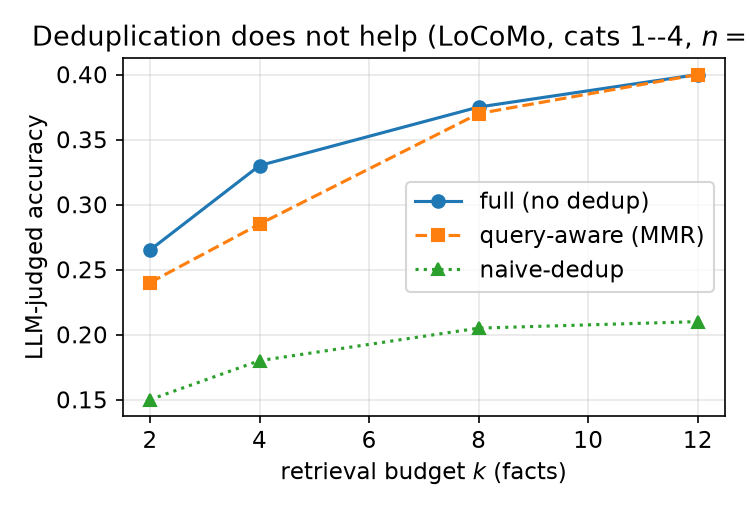
\includegraphics[width=\linewidth]{figures/fig_budget_sweep.png}
\caption{LLM-judged accuracy vs.\ retrieval budget. Naive deduplication is
dominated at every budget; redundancy-aware composition never exceeds plain
top-$k$.}
\label{fig:sweep}
\end{figure}

\begin{table}[t]
\centering
\small
\begin{tabular}{lcccc}
\toprule
policy & $k{=}2$ & $k{=}4$ & $k{=}8$ & $k{=}12$ \\
\midrule
full & 0.265 & 0.330 & 0.375 & 0.400 \\
naive-dedup & 0.150 & 0.180 & 0.205 & 0.210 \\
query-aware (MMR) & 0.240 & 0.285 & 0.370 & 0.400 \\
\bottomrule
\end{tabular}
\caption{LLM-judged accuracy vs.\ retrieval budget ($n{=}200$, categories 1--4).
Naive deduplication is dominated everywhere; redundancy-aware composition never
exceeds plain top-$k$.}
\label{tab:sweep}
\end{table}

\begin{table}[t]
\centering
\small
\begin{tabular}{lcc}
\toprule
policy & $k{=}8$ & $k{=}12$ \\
\midrule
full & 0.365 & 0.411 \\
naive-dedup & 0.152 & 0.163 \\
query-aware (MMR) & 0.358 & 0.433 \\
\midrule
\multicolumn{3}{l}{McNemar (query-aware vs.\ full):} \\
\multicolumn{3}{l}{\quad $k{=}8$: $b{=}31,c{=}33,\ p{=}0.90$ (n.s.)} \\
\multicolumn{3}{l}{\quad $k{=}12$: $b{=}29,c{=}23,\ p{=}0.49$ (n.s.)} \\
\bottomrule
\end{tabular}
\caption{Multi-hop (category 1), all $n{=}282$ questions. Redundancy-aware
composition is statistically indistinguishable from plain top-$k$; naive
deduplication remains dominated.}
\label{tab:multihop}
\end{table}

\paragraph{Takeaway.} On this pipeline, deduplication is not a useful lever:
blind merging harms accuracy, and redundancy-aware selection is safe but
inert. If accuracy is being lost, it is being lost elsewhere.
